\newpage
\section{Νευρωνικά Δίκτυα}
Τα νευρωνικά δίκτυα είναι στις μέρες μας το κυρίαρχο μοντέλο στη μηχανική μάθηση και μπορεί να λύσει και τους τρεις τύπους προβλημάτων που έχουμε δει (ταξινόμηση, παλινδρόμηση και ομαδοποίηση). Τα τεχνητά νευρωνικά δίκτυα δημιουργήθηκαν με
σκοπό να μιμηθούν τον τρόπο που λειτουργεί ο εγκέφαλος του ανθρώπου. Οι νευρώνες του εγκεφάλου μας λειτουργούν δημιουργώντας συνδέσεις με άλλους νευρώνες και όλοι μαζί συμβάλουν στην επεξεργασία ενός ηλεκτρικού σήματος που έρχεται από τον
εγκέφαλο το οποίο τελικά καταλήγει να είναι απλή καθημερινή πράξη για τον άνθρωπο (όπως για παράδειγμα να κουνήσει το χέρι του)\cite{nnip}.

Τα τεχνητά νευρωνικά δίκτυα προσπαθούν λοιπόν να αντιγράψουν αυτη ακριβώς την ιδιότητα. Ο σκοπός τους είναι να παίρνουν μια είσοδο και να παράγουν μία απάντηση. Για παράδειγμα θα μπορούσαμε σαν είσοδο να δώσουμε τις αιματολογικές εξετάσεις
ενός ανθρώπου και η έξοδος να είναι 0 ή 1 ανάλογα αν έχει μια ασθένεια ή όχι. Αυτό είναι ένα πρόβλημα δυαδικής ταξινόμησης αλλά θα μπορούσαμε να λύσουμε και πολλά άλλα προβλήματα και θα αναλύσουμε στην συνέχεια τις αλλαγές που πρέπει να
κάνουμε σε ένα νευρωνικό δίκτυο ανάλογα το πρόβλημα. Σε αυτή την ενότητα θα αναλύσουμε διάφορες έννοιες τις οποίες πρέπει να γνωρίζει κανείς αν θέλει να κατανοήσει τα νευρωνικά δίκτυα. Αυτές είναι\cite{nnav}:
\begin{itemize}
    \item Νευρώνας
    \item Επίπεδο
    \item Οπισθοδρόμηση (\en{back propagation})
    \item Συναρτήσεις ενεργοποίησης
    \item Συναρτήσεις σφάλματος
\end{itemize}
\subsection{Επίπεδα}
Το απλούστερο δίκτυο νευρώνων αποτελείται από 3 ήδη επιπέδων, το επίπεδο εισόδου(\en{input layer}),
το κρυφό επίπεδο(\en{hidden layer}) και το επίπεδο εξόδου(\en{output layer}).

% picture

Στο επίπεδο εισόδου ο κάθε νευρώνας έχει τις τιμές της εισόδου (π.χ. για εικόνα τις \en{RGB} τιμές
κάθε \en{pixel}) και έχει όσους νευρώνες όσες και οι χαρακτηριστικές τιμές της εισόδου. Στο
επίπεδο εξόδου συνήθως υπάρχουν τόσοι νευρώνες όσα και τα αντικείμενα που θέλουμε να
αναγνωρίζει, αλλά αυτό εξαρτάται από την κωδικοποίηση που θα χρησιμοποιήσουμε.

Το
κρυφό επίπεδο μπορεί να έχει αυθαίρετο αριθμό νευρώνων και είναι κάτι που αποφασίζει ο χρήστης
σύμφωνα με το πρόβλημα και με τον όγκο πληροφορίας που έχει στην διάθεσή του. Συνήθως
οι περισσότεροι νευρώνες οδηγούν σε πιο ακριβή προβλέψεις, αλλά ταυτόχρονα αυξάνουν
την πολυπλοκότητα και το υπολογιστικό κόστος.

Σε μεγαλύτερα δίκτυα ο μεγάλος αριθμός
νευρώνων σε ένα επίπεδο μπορεί να οδηγήσει σε ένα φαινόμενο που λέγεται \en{over-fitting} το οποίο
θα αναλυθεί αργότερα. Παράλληλα με τον αριθμό των νευρώνων μπορεί να υπάρχουν
πολλαπλά κρυφά επίπεδα, με διαφορετικό αριθμό νευρώνων ο καθένας, και ο αριθμός τους
βελτιστοποιείται και αυτός σύμφωνα με το μέγεθος του προβλήματος και τον όγκο των
δεδομένων.

Συνήθως στα πιο απλά δίκτυα οι νευρώνες κάθε επιπέδου συνδέονται με όλους τους
νευρώνες του επόμενου, με ξεχωριστά βάρη για κάθε σύναψη, σχηματίζοντας ένα πλήρως
συνδεδεμένο(\en{fully connected}) ή πυκνό (\en{dense}) επίπεδο. Με αυτό τον τρόπο η έξοδος των
προηγούμενων επιπέδων αποτελεί την είσοδο των επόμενων. Ανάλογα με την υλοποίηση
μπορούν να χρησιμοποιηθούν και άλλα είδη επιπέδων αλλά δεν θα τα αναλύσουμε στην
παρούσα εργασία. Αναφορικά μερικά από τα επίπεδα που μπορούμε να χρησιμοποιήσουμε
είναι:
\begin{itemize}
    \item \en{Convolutional}
    \item \en{Max Pooling}
    \item \en{Flatten}
    \item \en{Batch Normalization}
    \item \en{Dropout}
    \item \en{Residual}
\end{itemize}

Τα βάρη είναι οι τιμές που εκπαιδεύουμε και λέγονται έτσι καθώς μας δείχνουν πόσο βάρος
(έμφαση) πρέπει να δώσουμε στην κάθε είσοδο (έξοδο του προηγούμενου επιπέδου). Η
συνολική είσοδος που "βλέπει" ο νευρώνας υπολογίζεται από το σταθμισμένο άθροισμα
όλων των εισόδων και μίας τιμής bias που επηρεάζει την πρόβλεψη του νευρώνα:
$$S_{in}=\sum\limits_{i=0}^na_iw_i+b$$
Η τιμή του νευρώνα προκύπτει από τιμή της συνάρτησης ενεργοποίησης όταν έχει για είσοδο
το σταθμισμένο άθροισμα:
$$a=f(S_{in})$$
Η αρχικοποίηση των βαρών γίνεται με τυχαίο τρόπο και με την πάροδο του χρόνου, μέσω της
διαδικασίας της εκπαίδευσης, συγκλίνουν στις κατάλληλες τιμές.

Για να εκπαιδεύσουμε το δίκτυο χρησιμοποιούμε δύο μεθόδους που λέγονται \en{forward} και
\en{back propagation} και θα αναλυθούν λεπτομερώς παρακάτω. Με τις δύο μεθόδους περνάμε
τα δεδομένα μας πολλές φορές από το δίκτυο μέχρι αυτό να εκπαιδευτεί επαρκώς. Σύμφωνα
με κάποια κριτήρια μπορεί να τερματίσουμε την εκπαίδευση πρόωρα για να διασφαλίσουμε
την ακρίβεια των προβλέψεων που κάνουμε.
\subsection{Διάδοση προς τα εμπρός}
Έχοντας λοιπόν το απλό νευρωνικό δίκτυο με 1 input, 1 hidden και 1 output layer, όπου όλα
μεταξύ τους είναι fully connected, θα αναλύσουμε τον τρόπο με τον οποίο διαδίδεται η
πληροφορία από τα πίσω προς τα μπροστά επίπεδα, δηλαδή από την είσοδο προς την έξοδο.

Για να ξεκινήσουμε θα αριθμήσουμε όλους τους νευρώνες του δικτύου. Οι εκθέτες δείχνουν
το επίπεδο που είμαστε με τα \en{input} να είναι το επίπεδο 0. Οι δείκτες δίνουν τον αριθμό του
νευρώνα στο εκάστοτε επίπεδο. Έτσι λοιπόν θα ξεκινήσουμε από το επίπεδο 1 (1ο \en{hidden layer}),
εφόσον στο πρώτο δεν γίνεται κάποια διαδικασία υπολογισμού. Για τον νευρώνα $a_1^{[1]}$
η τιμή του υπολογίζεται περνώντας το σταθμισμένο άθροισμα όλων των εισόδων του από
την συνάρτηση ενεργοποίησης ως εξής:
$$a_1^{[1]}=f_A\left(\sum\limits_{i=1}^3\left[ w_{1i}^{[1]}\times a_i^{[0]}\right]+b_1\right)=f_A\left( w_{11}^{[1]}\times a_1^{[0]}+w_{12}^{[1]}\times a_2^{[0]}+w_{13}^{[1]}\times a_3^{[0]}+b_1\right)$$
Αντίστοιχα για το $a_2^{[1]}$
θα είχαμε:
$$a_2^{[1]}=f_A\left(\sum\limits_{i=1}^3\left[ w_{2i}^{[1]}\times a_i^{[0]}\right]+b_2\right)=f_A\left( w_{21}^{[1]}\times a_1^{[0]}+w_{22}^{[1]}\times a_2^{[0]}+w_{23}^{[1]}\times a_3^{[0]}+b_2\right)$$
Και ούτω καθεξής. Η σχέση αυτή γενικεύεται για $k$ επίπεδα και $n$ νευρώνες του κάθε
επιπέδου:
$$a_j^{[k]}=f_A\left(\sum\limits_{i=1}^n\left[ w_{ji}^{[k]}\times a_i^{[k-1]}\right]+b_j\right)$$
Όπου $j$ ο νευρώνας του επιπέδου που υπολογίζουμε την τιμή του με $j \in [1, n]$

Για την ευκολία υπολογισμού των πράξεων και αποθήκευσης από ένα υπολογιστικό σύστημα
θα μετατρέψουμε την παραπάνω σχέση σε μορφή πινάκων. Έτσι για την γενικευμένη
περίπτωση θα έχουμε:
$$
A^{[k]}=f_A\left(
\begin{bmatrix}
    w_{11}     & \dots     & w_{1n^{[k-1]}} \\
    \vdots     & \ddots    & \vdots \\
    w_{n^{[k]}1}   & \dots     & w_{n^{[k]}n^{[k-1]}}
\end{bmatrix}
^{[k]}
\times
\begin{bmatrix}
    a_1 \\
    \vdots \\
    a_{n^{[k-1]}}
\end{bmatrix}
^{[k]}
+
\begin{bmatrix}
    b_1 \\
    \vdots \\
    b_{n^{[k]}}
\end{bmatrix}
^{[k]}
\right)
=
\begin{bmatrix}
    a_1 \\
    \vdots \\
    a_{n^{[k]}}
\end{bmatrix}
^{[k]}
$$
Και απλοποιείται σε:
$$A^{[k]}=f_A(W^{[k]}\times A^{[k-1]}+B^{[k]})$$

Όπως βλέπουμε οι έξοδοι των νευρώνων από κάθε επίπεδο είναι είσοδοι για το επόμενο,
όπου με τον πολλαπλασιασμό των βαρών του επόμενου και το σταθμισμένο άθροισμα αυτών
($+$ το \en{bias} του επιπέδου), διαδίδουμε την πληροφορία προς τα μπροστά επίπεδα. Η
διαδικασία συνεχίζεται μέχρι να φτάσουμε στο τελευταίο επίπεδο (επίπεδο εξόδου), όπου
και παίρνονται οι αποφάσεις (προβλέψεις) με τον τρόπο που θα δούμε παρακάτω. Λόγο της
μετάδοσης αυτής προς τα εμπρός επίπεδα η διαδικασία ονομάζεται \en{forward propagation}.
\subsection{Οπισθοδρόμηση}

\subsection{Συναρτήσεις ενεργοποίησης}
Οι συναρτήσεις ενεργοποίησης είναι ένα πολύ σημαντικό κομμάτι των νευρωνικών δικτύων διότι προσφέρουν μη γραμμικότητα (επιθυμητή) στο σύστημά μας. Για να καταλάβουμε καλύτερα τι σημαίνει αυτό θα δούμε ένα παράδειγμα\cite{nnactmlm}:

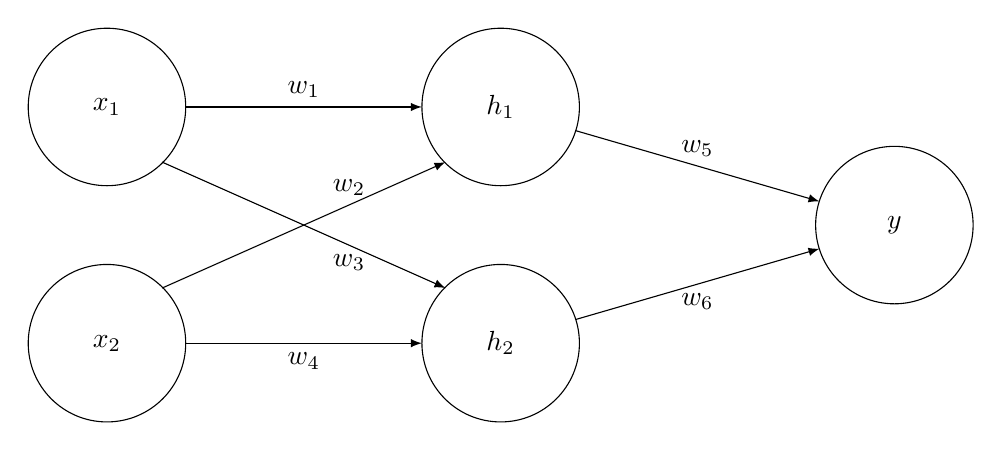
\begin{tikzpicture}
    \draw (0,0) circle (1) node{$x_2$};
    \draw (0,3) circle (1) node{$x_1$};
    \draw (5,0) circle (1) node{$h_2$};
    \draw (5,3) circle (1) node{$h_1$};
    \draw (10,1.5) circle (1) node{$y$};

    \draw[-latex] (1,0) -- (4,0) node[midway, below]{$w_4$};
    \draw[-latex] (1,3) -- (4,3) node[midway, above]{$w_1$};

    \draw[-latex] (0.7,0.7) -- (4.3,2.3) node[midway, above right=7]{$w_2$};
    \draw[-latex] (0.7,2.3) -- (4.3,0.7) node[midway, below right=7]{$w_3$};

    \draw[-latex] (5.95,2.7) -- (9.05,1.8) node[midway, above]{$w_5$};
    \draw[-latex] (5.95,0.3) -- (9.05,1.2) node[midway, below]{$w_6$};
\end{tikzpicture}

Βλεπουμε ότι η είσοδος με την έξοδο συνδέονται μέσω ενός κρυφού επιπέδου (\en{dense}) όπου:
\begin{gather*}
    h_1=w_1\times x_1+w_2\times x_2 \\
    h_2=w_3\times x_1+w_4\times x_2 \\
    y=w_5\times h_1+w_6\times h_2 \\
\end{gather*}
Αν αναλύσουμε λοιπόν τον τύπο του $y$ θα πάρουμε:
$$y=w_1(w_5\times x_1+w_2\times x_2) + w_6(w_3\times x_1+w_4\times x_2)$$
Που τελικά γίνεται:
$$y=(w_1w_5+w_3w_6)\times x_1+(w_2w_5+w_4w_6)\times x_2$$
Τα $w$ είναι σταθεροί αριθμοί οπότε τελικά ενώ έχουμε ένα κρυφό επίπεδο ανάμεσα στην είσοδο και στην έξοδο αυτές συνδέονται και πάλι με γραμμική σχέση. Το ίδιο θα συνέβαινε και για πολλαπλά κρυφά επίπεδα με πολλούς νευρώνες. Αυτό για το
δίκτυο μας σημαίνει ότι μπορεί να προσεγγίσει δεδομένα που ακολουθούν επίσης μια γραμμική σχέση. Τα δεδομένα όμως συνήθως δεν έχουν τέτοια συμπεριφορά. Για να λύσουμε αυτό το πρόβλημα δημιουργήθηκαν οι συναρτήσεις ενεργοποίησης. Στο
παράδειγμά μας μπορούμε να προσθέσουμε μις συνάρτηση ενεργοποίησης αμέσως μετά το κρυφό επίπεδο. Έτσι τελικά η έξοδος θα είναι:
$$y=w_5\times f_A(h_1)+w_6\times f_A(h_2)$$
Όπου $f_A$ η συνάρτηση ενεργοποίησης. Παρατηρούμε ότι η είσοδος δεν μπορεί πλέον να συνδεθεί γραμμικά με την έξοδο και άρα έχουμε πετύχει τον στόχο μας.

Υπάρχουν πολλές συναρτήσεις ενεργοποίησης και όλες έχουν τα πλεονεκτήματα και τα μειονεκτήματα τους. Εμεις θα αναλύσουμε κάποιες από τις πιο γνωστές οι οποίες χρησιμοποιούνται σχεδόν πάντα στα νευρωνικά δίκτυα.
Από τις πρώτες συναρτήσεις ενεργοποίησης ήταν η βηματική συνάρτηση:
\[f(x)=\left\{\begin{array}{ll}0 & x<0 \\ 1 & x>=0 \\ \end{array} \right.\]
\begin{figure}[H]
    \centering
    \begin{tikzpicture}
    \begin{axis}[axis lines=middle, xlabel=$x$, ylabel=$y$, xmin = -5, xmax=5, ymin=0, ymax=2, xtick={-5,-4,...,5}, ytick={0,1,2}]
        \addplot[color=red, domain=0:10]{1};
        \addplot[color=red, domain=-10:0]{0};
    \end{axis}
    \end{tikzpicture}
    \caption{\en{step function}}
\end{figure}
Η βηματική συνάρτηση είναι χρήσιμη όταν έχουμε ένα πρόβλημα δυαδικής ταξινόμησης. Μπορούμε δηλαδή να την εφαρμόσουμε στο επίπεδο εξόδου έτσι ώστε η απάντηση που θα παίρνουμε να είναι πάντα  0 ή 1. Όμως έχει ένα μεγάλο μειονέκτημά το οποίο
είναι ότι δεν είναι συνεχής. Η τεχνική της Οπισθοδρόμησης βασίζεται στις παραγώγους των συναρτήσεων κάτι το οποίο την κάνει πολύ δύσχρηστη. Θα μπορούσαμε θεωρητικά να αγνοήσουμε το 0 στο οποίο η συνάρτηση δεν είναι παραγωγίσιμη και να του
δώσουμε μια τιμή (όπως 0) αλλά υπάρχει ένα ακόμα πρόβλημα. Το πρόβλημα είναι ότι η παράγωγός της είναι παντού 0 και γνωρίζουμε από την οπισθοδρόμηση ότι πρέπει να πολλαπλασιάσουμε το σφάλμα με αυτή την παράγωγο. Άρα τελικά το σφάλμα που θα διαδίδεται στα επίπεδα θα είναι μηδενικό και άρα δεν θα γίνεται καμία διόρθωση.

Μια καλύτερη συνάρτηση που διατηρεί τα χαρακτηριστικά της βηματικής είναι η σιγμοειδής:
$$f(x)=\frac{1}{1+e^{-x}}$$
\begin{figure}[H]
    \centering
    \begin{tikzpicture}
    \begin{axis}[axis lines=middle, xlabel=$x$, ylabel=$y$, xmin = -5, xmax=5, ymin=0, ymax=2, xtick={-5,-4,...,5}, ytick={0,1,2}]
        \addplot[color=red]{exp(x)/(exp(x)+1)};
    \end{axis}
    \end{tikzpicture}
    \caption{\en{sigmoid function}}
\end{figure}
Αυτή η συνάρτηση είναι επίσης φραγμένη από το 0 ως το 1 και για αυτό μπορεί να χρησιμοποιηθεί επίσης στο επίπεδο εξόδου για δυαδική ταξινόμηση. Η σιγμοειδής όμως έχει ποιο ομαλή και συνεχή μετάβαση από το 0 στο 1 άρα μπορούμε να εφαρμόσουμε
τους κανόνες της οπισθοδρόμησης. Χρησιμοποιείται λοιπόν με αυτόν τον τρόπο μέχρι και σήμερα. Παρ' όλα αυτά για τα κρυφά επίπεδα, τα οποία δεν είναι απαραίτητο να κυμαίνονται απο 0 μέχρι 1, υπάρχει μια ακόμα καλύτερη συνάρτηση. Αυτή είναι η
συνάρτηση της υπερβολικής εφαπτομένης:
$$f(x)=\tanh (x)=\frac{e^x-e^{-x}}{e^x+e^{-x}}$$
\begin{figure}[H]
    \centering
    \begin{tikzpicture}
    \begin{axis}[axis lines=middle, xlabel=$x$, ylabel=$y$, xmin = -5, xmax=5, ymin=-2, ymax=2, xtick={-5,-4,...,5}, ytick={-2,-1,...,2}]
        \addplot[color=red]{tanh(x)};
    \end{axis}
    \end{tikzpicture}
    \caption{\en{tanh function}}
\end{figure}
Η συνάρτηση αυτή είναι καλύτερη επειδή αντιμετωπίζει το λεγόμενο \en{vanishing gradient problem}. Για να καταλάβουμε τι σημαίνει αυτό θα πρέπει να συγκρίνουμε τις παραγώγους των δύο συναρτήσεων:
\begin{figure}[H]
    \centering
    \begin{subfigure}{0.49\textwidth}
        \centering
        \begin{tikzpicture}
        \begin{axis}[axis lines=middle, xlabel=$x$, ylabel=$y$, xmin = -5, xmax=5, ymin=0, ymax=1, xtick={-5,-4,...,5}, ytick={0,0.25,...,1}]
            \addplot[color=red]{(exp(x)/(exp(x)+1))*(1-(exp(x)/(exp(x)+1)))};
        \end{axis}
        \end{tikzpicture}
        \caption{\en{sigmoid derivative}}
    \end{subfigure}
    \begin{subfigure}{0.49\textwidth}
        \centering
        \begin{tikzpicture}
        \begin{axis}[axis lines=middle, xlabel=$x$, ylabel=$y$, xmin = -5, xmax=5, ymin=0, ymax=1, xtick={-5,-4,...,5}, ytick={0,0.25,...,1}]
            \addplot[color=red]{1-tanh(x)^2};
        \end{axis}
        \end{tikzpicture}
        \caption{\en{tanh derivative}}
    \end{subfigure}
    \caption{\en{derivative comparison}}
\end{figure}
Από το παραπάνω σχήμα μπορούμε να δούμε ότι η παράγωγός της σιγμοειδούς έχει μέγιστη τιμή το 0.25. Αυτό σημαίνει ότι αν έχουμε πολλά κρυφά επίπεδα με αυτή την ενεργοποίηση, κάθε φορά που το σφάλμα θα διαδίδεται από το ένα επίπεδο στο άλλο
θα υπο-τετραπλασιάζεται στην καλύτερη περίπτωση. Έτσι στο τέλος τα αρχικά επίπεδα θα κάνουν ελάχιστη διόρθωση στα βάρη τους. Αντιθέτως η παράγωγος της υπερβολικής εφαπτομένης έχει μέγιστο το 1 άρα δίνει πολύ καλύτερα αποτελέσματα. Παρ' ότι
μειώνεται το πρόβλημα όμως δεν εξαφανίζεται. Γι' αυτό οι επόμενες συναρτήσεις που θα δούμε αντιμετωπίζουν πλήρως το \en{vanishing gradient problem}.

Η επόμενη συνάρτηση που αυτή τη στιγμή είναι και η πιο διάσημη συνάρτηση ενεργοποίησης στη μηχανική μάθηση είναι η \en{ReLU (rectified linear unit)}:
\[f(x)=\left\{\begin{array}{ll}0 & x<0 \\ x & x>=0 \\ \end{array} \right.\]
\begin{figure}[H]
    \centering
    \begin{tikzpicture}
    \begin{axis}[axis lines=middle, xlabel=$x$, ylabel=$y$, xmin = -5, xmax=5, ymin=0, ymax=5, xtick={-5,-4,...,5}, ytick={0,1,...,5}, axis equal]
        \addplot[color=red, domain=0:10]{x};
        \addplot[color=red, domain=-10:0]{0};
    \end{axis}
    \end{tikzpicture}
    \caption{\en{ReLU function}}
\end{figure}
Η συνάρτηση αυτή έχει την ικανότητα να προσφέρει ταυτόχρονα τα πλεονεκτήματα της γραμμικότητας αλλά και της μη γραμμικότητας. Λόγω της γραμμικότητας δεν έχει το \en{vanishing gradient problem} και επίσης έχει πολύ απλή υλοποίηση. Αλλά η μη
γραμμικότητα που έχει της επιτρέπει να εφαρμόζει την επιθυμητή μη γραμμικότητα που θέλουμε στα νευρωνικά δίκτυα. Ενώ η συνάρτηση είναι η πιο διάσημη δεν σημαίνει ότι δεν έχει και αυτή τα προβλήματά της. Συγκεκριμένα μιλάμε για το λεγόμενο
\en{dying ReLU problem}. Συγκεκριμένα η παράγωγός της για αρνητικές τιμές είναι 0. Αυτό σημαίνει ότι όταν είναι αρνητική η είσοδος δεν θα μπορεί να διαδοθεί το σφάλμα από εκείνο το επίπεδο. Γι' αυτό και οι επόμενες συναρτήσεις που θα δούμε
είναι παραλλαγές αυτής της συνάρτησης με σκοπό να αντιμετωπίσουν αυτό το πρόβλημα. Ξεκινάμε με την \en{Leaky ReLU}:
\[f(x)=\left\{\begin{array}{ll}0.01x & x<0 \\ x & x>=0 \\ \end{array} \right.\]
\begin{figure}[H]
    \centering
    \begin{tikzpicture}
    \begin{axis}[axis lines=middle, xlabel=$x$, ylabel=$y$, xmin = -5, xmax=5, ymin=0, ymax=5, xtick={-5,-4,...,5}, ytick={0,1,...,5}, axis equal]
        \addplot[color=red, domain=0:10]{x};
        \addplot[color=red, domain=-10:0]{0.1*x};
    \end{axis}
    \end{tikzpicture}
    \caption{\en{ReLU function}}
\end{figure}
Γενίκευση της αποτελει τη \en{parametric ReLU} με τύπο:
\[f(x)=\left\{\begin{array}{ll}ax & x<0 \\ x & x>=0 \\ \end{array} \right.\]
Αυτές αντιμετωπίζουν το πρόβλημα με έναν πολύ απλό τρόπο. Παρ' όλα αυτά έχουν βρεθεί και πιο πολύπλοκες συναρτήσεις που θα δούμε παρακάτω. Ακολουθεί η συνάρτηση \en{ELU (exponential linear unit)}:
\[f(x)=\left\{\begin{array}{ll}a(e^x-1) & x<0 \\ x & x>=0 \\ \end{array} \right.\]
\begin{figure}[H]
    \centering
    \begin{tikzpicture}
    \begin{axis}[axis lines=middle, xlabel=$x$, ylabel=$y$, xmin = -5, xmax=5, ymin=0, ymax=5, xtick={-5,-4,...,5}, ytick={0,1,...,5}, axis equal]
        \addplot[color=red, domain=0:10]{x};
        \addplot[color=red, domain=-10:0]{(exp(x)-1)};
    \end{axis}
    \end{tikzpicture}
    \caption{\en{ELU function}}
\end{figure}
Όπως και πριν μπορούμε να γενικεύσουμε αυτή τη συνάρτηση. Η γενικευμένη μορφή ονομάζεται \en{SELU (scaled exponential linear unit)}:
\[f(x)=\lambda\left\{\begin{array}{ll}a(e^x-1) & x<0 \\ x & x>=0 \\ \end{array} \right.\]
\begin{figure}[H]
    \centering
    \begin{tikzpicture}
    \begin{axis}[axis lines=middle, xlabel=$x$, ylabel=$y$, xmin = -5, xmax=5, ymin=-5, ymax=5, xtick={-5,-4,...,5}, ytick={0,1,...,5}, axis equal]
        \addplot[color=red, domain=0:10]{x};
        \addplot[color=red, domain=-10:0]{2*(exp(x)-1)};
    \end{axis}
    \end{tikzpicture}
    \caption{\en{SELU function}}
\end{figure}
Οι παραπάνω συναρτήσεις όπως έχουμε δει έχουν δύο κλάδους με σκοπό να πετύχουν τη γραμμικά και μη γραμμικά στοιχεία που θέλουμε. Οι παρακάτω συναρτήσεις καταφέρνουν να έχουν παρόμοια συμπεριφορά με έναν τύπο συνάρτησης. Η μία από αυτές
είναι η \en{GELU (Gaussian error linear unit)}:
$$0.5x\left(1+\tanh \left[\frac{\sqrt{2}}{\pi}(x+0.044715x^3)\right]\right)$$
\begin{figure}[H]
    \centering
    \begin{tikzpicture}
    \begin{axis}[axis lines=middle, xlabel=$x$, ylabel=$y$, xmin = -5, xmax=5, ymin=0, ymax=5, xtick={-5,-4,...,5}, ytick={0,1,...,5}, axis equal]
        \addplot[color=red]{0.5*x*(1+tanh(sqrt(2)/pi*(x+0.044715*x^3)))};
    \end{axis}
    \end{tikzpicture}
    \caption{\en{GELU function}}
\end{figure}
Η δεύτερη συνάρτηση είναι η συνάρτηση \en{swish}:
$$f(x)=\frac{x}{1+e^{-x}}$$
\begin{figure}[H]
    \centering
    \begin{tikzpicture}
    \begin{axis}[axis lines=middle, xlabel=$x$, ylabel=$y$, xmin = -5, xmax=5, ymin=-2, ymax=2, xtick={-5,-4,...,5}, ytick={0,1,2}, axis equal]
        \addplot[color=red]{x/(exp(-x)+1)};
    \end{axis}
    \end{tikzpicture}
    \caption{\en{swish function}}
\end{figure}
Όλες αυτές οι συναρτήσεις έχουν παρόμοιες ιδιότητες. Πολλές από αυτές θεωρητικά μπορεί να είναι καλύτερες από τη \en{ReLU} αλλά στην πράξη αυτή εξακολουθεί να είναι η κυρίαρχη συνάρτηση για λόγους απλότητας.

Όλες οι συναρτήσεις που έχουμε δείξει μέχρι τώρα με εξαίρεση την σιγμοειδή χρησιμοποιούνται μόνο σε κρυφά επίπεδα. Παρ' όλα αυτά χρειαζόμαστε και κάποιες συναρτήσεις για τα επίπεδα εξόδου οι οποίες να ευνοούν το πρόβλημα που έχουμε να
λύσουμε. Για παράδειγμα όπως έχουμε ήδη αναφέρει, για ένα πρόβλημα δυαδικής ταξινόμησης θα χρησιμοποιούσαμε τη σιγμοειδή συνάρτηση. Το ίδιο ισχύει και για ένα πρόβλημα ταξινόμησης πολλών ετικετών. Θα είχαμε δηλαδή πολλούς νευρώνες στην
έξοδο και καθένας απο αυτους θα χρησιμοποιούσε τη σιγμοειδή σαν συνάρτηση ενεργοποίησης.

Τα προβλήματα τα οποία παραμένουν είναι η παλινδρόμηση και η ταξινόμηση πολλαπλών κλάσεων (αλλά μόνο μία ετικέτα τη φορά). Η συνάρτηση ενεργοποίησης που Χρησιμοποιείται στην παλινδρόμηση είναι η γραμμική συνάρτηση:
$$f(x)=\lambda x$$
\begin{figure}[H]
    \centering
    \begin{tikzpicture}
    \begin{axis}[axis lines=middle, xlabel=$x$, ylabel=$y$, xmin = -5, xmax=5, ymin=-2, ymax=2, xtick={-5,-4,...,5}, ytick={-2,-1,...,2}, axis equal]
        \addplot[color=red]{x};
    \end{axis}
    \end{tikzpicture}
    \caption{\en{linear function}}
\end{figure}
Αυτή η συνάρτηση βρίσκει χρήση μόνο σε επιπεδα εξόδου. Οι συναρτήσεις που έχουμε δείξει μέχρι στιγμής είναι όλες φραγμένες από μία ή και από δύο μεριές. Αυτό τις καθιστά ακατάλληλες για την εφαρμογή στην έξοδο ενός προβλήματος
παλινδρόμησης στο οποίο η έξοδος θα πρέπει να μπορεί να πάρει οποιαδήποτε τιμή. Γι' αυτό και υπάρχει η γραμμική συνάρτηση για αυτές τις περιπτώσεις.

Τέλος μας μένει το πρόβλημα ταξινόμησης πολλαπλών κλάσεων. Θα μπορούσε να λυθεί με τον ίδιο τρόπο με το πρόβλημα πολλαπλών ετικετών. Όμως σε αυτήν την περίπτωση δεν μας ενδιαφέρει δύο νευρώνες να μπορούν να τείνουν στην τιμή 1 αλλά μόνο
ένας τη φορά. Γι' αυτόν ακριβώς το λόγο υπάρχει μια καλύτερη συνάρτηση για αυτή τη δουλεια που λέγεται \en{softmax}:
$$f_i(x)=\frac{e^{x_i}}{\sum\limits_{k=1}^Ne^{x_k}}$$
$N$ είναι ο αριθμός των νευρώνων της εισόδου. Η συγκεκριμένη συνάρτηση όπως μπορεί να καταλάβει κανείς παράγει τιμές (όσοι και οι είσοδοι) που αθροίζονται σε 1. Ταυτόχρονα όμως επειδή χρησιμοποιούμε την εκθετική συνάρτηση οι μεγάλες τιμές
γίνονται ακόμα πιο μεγάλες (δηλαδή παίρνουν μεγαλύτερο ποσοστό). Επισης η εκθετική συνάρτηση μας βοηθάει και σε άλλα προβλήματα όπως με τις αρνητικές τιμές  και με μηδενικά αθροίσματα (διαίρεση με το 0).

\subsection{Συναρτήσεις κόστους}
Ένα ακόμα πολύ σημαντικό στοιχείο των νευρωνικών δικτύων είναι οι συναρτήσεις κόστους. Οι συναρτήσεις κόστους είναι αυτές που μας επιτρέπουν να αξιολογήσουμε την ποιότητα του δικτύου μας στο στάδιο της εκπαίδευσης αλλά και της επαλήθευσης.
Αυτό μπορεί να μας δώσει χρήσιμες πληροφορίες όπως για παράδειγμα αν υπάρχει \en{over fitting} (κάτι που θα σήμαινε ότι πρέπει να σταματήσουμε). Όπως είδαμε και με τις συναρτήσεις ενεργοποίησης υπάρχουν διαφορετικοί τύποι προβλήματος και
για τον καθένα από αυτούς είχαμε και μια διαφορετική ενεργοποίηση εξόδου που ήταν κατάλληλη για το συγκεκριμένο πρόβλημα. Το ίδο ακριβώς συμβαίνει και με τις συναρτήσεις κόστους.

Ξεκινώντας με το πιο απλό πρόβλημα της παλινδρόμησης έχουμε δύο συναρτήσεις κόστους οι οποίες είναι πολύ παρόμοιες. Αυτές είναι οι \en{mean absolute error (MAE)} και \en{mean square error (MSE)}:
\begin{gather*}
    \enm{MAE}=\frac{1}{N}\sum\limits_{i=1}^{N}\left\lvert y_i-p_i\right\rvert \\
    \enm{MSE}=\frac{1}{N}\sum\limits_{i=1}^{N}\left( y_i-p_i\right)^2
\end{gather*}
Όπου:
\begin{description}
    \item[$y$ :] Η έξοδος που παράχθηκε από το νευρωνικό δίκτυο
    \item[$p$ :] Η πραγματική έξοδος
\end{description}
Ό λόγος που θέλουμε να έχουμε απόλυτη τιμή ή τετράγωνο είναι διότι μπορεί να υπάρχει και αρνητικό σφάλμα, κάτι το οποίο θα οδηγούσε τα σφάλματα στο να αναιρούν το ένα το άλλο (τα θετικά και αρνητικά) και στο τέλος θα παίρναμε ένα σφάλμα το
οποίο δεν θα ήταν αντιπροσωπευτικό για το δίκτυο. Επίσης το \en{MSE} πολλές φορές προτιμάται λόγω του ότι είναι παραγωγίσιμη συνάρτηση.

Η επόμενη συνάρτηση κόστους που θα δούμε χρησιμοποιείται σε προβλήματα δυαδικής ταξινόμησης και λέγεται \en{binary cross entropy}:
$$C=-[p\log (y) + (1-p)\log (1-y)]$$
Για να καταλάβουμε πώς μπορεί να αντιπροσωπεύει το κόστος αυτή  η συνάρτηση θα δείξουμε κάποια παραδειγματα. Αρχικά το $p$ που είναι η πραγματική τιμή σε ένα πρόβλημα δυαδικής ταξινόμησης μπορεί να πάρει μόνο τις τιμές 0 ή 1. Αν λοιπόν
είναι 0 τότε έχουμε:
$$C=-\log (1-y)$$
\begin{figure}[H]
    \centering
    \begin{tikzpicture}
    \begin{axis}[axis lines=middle, xlabel=$x$, ylabel=$y$, xmin = -5, xmax=5, ymin=-2, ymax=5, xtick={-5,-4,...,5}, ytick={-2,-1,...,2}, axis equal]
        \addplot[color=red,samples=200]{-ln(1-x)};
        \addplot[mark=none, dashed] coordinates {(1, -2) (1, 5)};
    \end{axis}
    \end{tikzpicture}
    \caption{\en{binary error for $p=0$}}
\end{figure}
Μπορούμε από τη γραφική παράσταση να δούμε ότι αν το $x$ γίνει 0 (όσο και η πραγματική τιμή) τότε το σφάλμα γίνεται και αυτό 0 ενώ αν το $x$ τείνει στο 1 τότε το σφάλμα τείνει στο άπειρο.
Το αντιστοιχο συμβαίνει και για την περίπτωση που το $p$ είναι 1:
$$C=-\log (y)$$
\begin{figure}[H]
    \centering
    \begin{tikzpicture}
    \begin{axis}[axis lines=middle, xlabel=$x$, ylabel=$y$, xmin = -5, xmax=5, ymin=-2, ymax=5, xtick={-5,-4,...,5}, ytick={-2,-1,...,2}, axis equal]
        \addplot[color=red,samples=200]{-ln(x)};
    \end{axis}
    \end{tikzpicture}
    \caption{\en{binary error for $p=1$}}
\end{figure}
Με παρόμοιο τρόπο ορίζεται και η συνάρτηση κόστους για την ταξινόμηση πολλαπλών κλάσεων γνωστή και ως \en{categorical crossentropy}:
$$C=-\sum\limits_{i=1}^Np_i\log (y_i)$$
Οι πραγματική έξοδος $p$ σε αυτή την περίπτωση είναι ένα διάνυσμα που έχει παντου μηδενικά εκτός από μια τιμή που θα είναι 1. Αρα αν αυτή  η τιμή είναι το $p_k$ τότε έχουμε:
$$C=-\log (y_k)$$
Μπορούμε και εδώ να δούμε πως συμπεριφέρεται η συνάρτηση με τον ίδιο τρόπο που είδαμε στην δυαδική ταξινόμηση. Εδώ όμως αν παρατηρήσουμε η συνάρτηση έχει γίνει ανεξάρτητη όλων των άλλων εξόδων. Αν δηλαδή βγάζαμε μια έξοδο στην οποία όλες οι
τιμές είχαν την τιμή 1, τότε το κόστος θα ήταν μηδενικό (κάτι που προφανώς δεν ισχύει). Πρέπει όμως να θυμηθούμε ότι στα προβλήματα αυτού του είδους η συνάρτηση ενεργοποίησης της εξόδου είναι η συνάρτηση \en{softmax}. Αυτό σημαίνει ότι μια
τέτοια περίπτωση δεν μπορεί να συμβεί ποτέ. Βλέπουμε λοιπόν ότι μπορει να υπάρχει μια συνεργασία ανάμεσα στις ενεργοποιήσεις εξόδου και στις συναρτήσεις κόστους.

Τελευταίο είναι το πρόβλημα ταξινόμησης πολλαπλών ετικετών. Για αυτόν τον τύπο προβλήματος η συνάρτηση κόστους είναι ένας συνδυασμός των δύο προηγούμενων:
$$C=-\left[\sum\limits_{i=1}^Np_i\log (y_i) +\sum\limits_{i=1}^N(1-p_i)\log (1-y_i)\right]$$
Σε τέτοια προβλήματα χρησιμοποιούμε τη σιγμοειδή συνάρτηση σαν ενεργοποίηση εξόδου. Αυτό σημαίνει ότι δεν μπορούμε να έχουμε τις ίδιες ιδιότητες που είχε η συνάρτηση \en{softmax} οπότε πρέπει να έχουμε μια συνάρτηση κόστους που να λαμβάνει
υπόψη της τις τιμές όλων των νευρώνων. Εδώ η πραγματική έξοδος μπορεί να έχει την τιμή 1 σε πάνω από μία θέσεις αλλά για λόγους απλότητας θα εξετάσουμε και πάλι το παράδειγμα που μόνο το $p_k$ είναι 1:
$$C=-\left[\log (y_k) +\sum\limits_{i=1,i\neq k}^N\log (1-y_i)\right]$$
Έτσι μπορούμε να δούμε ότι αν κάποια τιμή που θα έπρεπε να είναι 0 τείνει στο 1 η το αντίστροφο το κόστος θα τείνει στο άπειρο ενώ αν οι τιμές είναι ίσες με τις πραγματικές τότε το κόστος είναι 0.